\section{EvalCourse}
En este trabajo hemos buscado literatura que aborde la evaluación de competencias genéricas, y a ser posible, que lo hagan de manera automática utilizando la interacción de los estudiantes con el LMS. En línea con este trabajo, y a fin de abordar lo que será mi futura tesis doctoral, estamos trabajando en una herramienta que cumpla este propósito. Esta herramienta, cuyo prototipo ya ha sido presentado en varios congresos \cite{Balderas:2013,Balderas:2013a}, se llama EvalCourse y su lógica viene descrita en la figura \ref{fig:EvalcourseLogica}. EvalCourse es un Lenguaje de Dominio Específico (DSL). Al tratarse de un proyecto open-source, todo el desarrollo de EvalCourse se lleva a cabo utilizando una forja de código libre \footnote{https://www.assembla.com/spaces/evalcourse}. Un DSL es un lenguaje de programación orientado a un problema específico y con una semántica orientada al dominio para el que se diseña. En nuestro caso, este dominio es la evaluación de indicadores de competencias de los estudiantes. Un ejemplo de funcionamiento puede verse en la figura \ref{fig:EvalCourseCodigo}. El objetivo de EvalCourse es ayudar al docente en la evaluación del desempeño de los alumnos en las competencias que éstos deben desarrollar a lo largo del curso. Estos datos deberán servir al docente como indicadores del desarrollo de dichas competencias. La idea inicial con la que se ha desarrollado este proyecto, es que el DSL sea genérico y pueda ser utilizado con otros sistemas, no sólo de tipo LMS, sino también con sistemas que fomenten el trabajo colaborativo, como pueden ser los wikis. De hecho, se ha desarrollado software para evaluar diversas competencias (tanto genéricas como específicas) mediante análisis de registro (StatMediaWiki) como entre pares o autoevaluaciones (AssessMediaWiki) \cite{Palomo-Duarte:2013}.



\begin{figure}[H]
  \begin{center}
    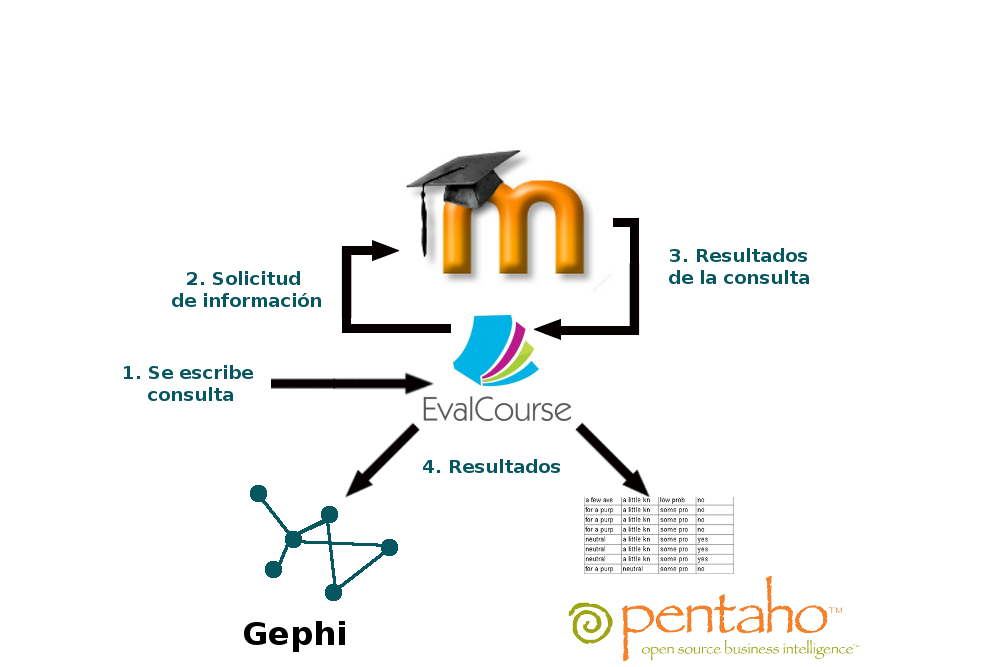
\includegraphics[scale=0.4]{cap5_evalcourse_logica.png}
  \end{center}
  \caption{Esquema lógico de EvalCourse}
  \label{fig:EvalcourseLogica}
\end{figure}


\begin{figure}[H]
  \begin{center}
    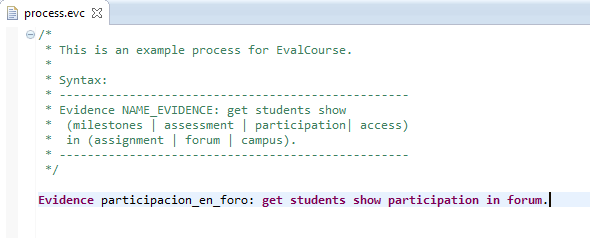
\includegraphics[scale=0.6]{cap5_evalcourse_codigo.png}
  \end{center}
  \caption{Consulta realizada en EvalCourse para obtener la participación en foros}
  \label{fig:EvalCourseCodigo}
\end{figure}

\section{Experiencia piloto}
Durante el presente curso 2013/14 se está desarrollando un proyecto financiado por la Convocatoria de Actuaciones Avaladas para la Mejora Docente, Formación del Profesorado y Difusión de Resultados con fondos de la Consejería de Economía, Innovación, Ciencia y Empleo de la Junta de Andalucía, con el título \emph{Extracción de indicadores objetivos para evaluación del desarrollo de competencias genéricas a partir de registros de actividad del Campus Virtual}. La Unidad de Innovación Docente de la Universidad de Cádiz concedió dicha actuación con código \emph{AAA\_14\_009} y actualmente se está desarrollando. En ella participan 8 profesores de 6 asignaturas del Grado en Ingeniería Informática.

Este proyecto se engloba dentro del trabajo realizado dentro del grupo de investigación SPI\&FM (TIC-195) por parte de Antonio Balderas al uso de las tecnologías en los entornos de aprendizaje. Se pretende desarrollar y aplicar EvalCourse, un DSL que permita a los docentes mediante el uso de una sintaxis sencilla obtener indicadores del desempeño de los estudiantes en diferentes competencias. Son varias las asignaturas de Grado en Ingeniería Informática que participan en este proyecto. Las tareas que comprende son:

\begin{enumerate}
\item Analizar los tipos de indicadores que se podrían obtener de la base de datos Moodle que sean de utilidad para los profesores, así como la manera de obtenerlos.
\item Análisis, desarrollo y prueba del software. Implementar el software DSL para que se conecte a Moodle y pueda extraer la información. Para ello sería necesario la instalación de un entorno de pruebas Moodle y la generación de una batería de datos de pruebas que permita verificar el funcionamiento del software.
\item Obtención de datos reales de las asignaturas del campus virtual. A partir de estos, utilizaremos la herramienta para obtener todos los indicadores necesarios para evaluar las competencias de los estudiantes. Además podremos corregir aquellos fallos que se detecten en el software.
\item Análisis de resultados de la experiencia, difusión del trabajo realizado, publicación de informes, correcciones menores en el sistema, etc. Se analizarán los resultados obtenidos y se darán a conocer el software y la experiencia en webs especializadas, redes sociales, etc. Igualmente se procederá a la correcta documentación del sistema en una web oficial para poder replicar la experiencia (incidiendo en cómo evitar los errores cometidos), así como pequeños desarrollos que corrijan deficiencias observadas y faciliten la reutilización del sistema.
\end{enumerate}

\section{Trabajo futuro} % Creada sección debido a comentario 89, pero hay que cambiar más. Esperar comentarios Juanma.
El trabajo futuro no es otro que afrontar el desarrollo de mi tesis doctoral. Partimos de las bases sentadas en este trabajo de investigación, habiendo analizado la situación actual de la evaluación de competencias genéricas. Los próximos pasos de esta línea, pasan por seleccionar, por un lado, varios entornos virtuales. Pero estos entornos virtuales ya no serán sólo en Moodle, como han sido las experiencias piloto desarrolladas en los artículos \cite{Balderas:2013,Balderas:2013a}, sino ampliar a otros LMS, a wikis y CMS (Content content Management System). Ya en el curso pasado se realizó una experiencia basada en \emph{AssessMediaWiki} \cite{Balderas:2012}, en el que se utilizaban los registros de un wiki basado en \emph{MediaWiki} para que, mediante evaluación entre iguales, los estudiantes analizasen las diferencias entre los trabajos de dos compañeros. Por tanto, y aunque con otro fin, ya se ha realizado una inmersión a la extracción de datos a partir de los registros del wiki.

Por otro lado, el trabajo futuro se ha de probar con diferentes cursos que cuenten con un alto número de estudiantes, demostrando que este método de evaluación es sostenible, y que además, el método no sufre al incrementar la cantidad de alumnos, validando así su escalabilidad.

Desglosando el párrafo anterior, nos encontramos ante un doble objetivo general como trabajo futuro:
\begin{itemize}
\item Objetivo funcional: ser capaz de recoger información de una diversidad de sistemas: LMS, wikis y CMS.
\item Objetivo no funcional: ser capaz de evaluar el desempeño de los alumnos en el sistema, a pesar de que el número de alumnos sea muy elevado.
\end{itemize}



